%# -*- coding: utf-8-unix -*-
%%==================================================
%% chapter01.tex for SJTU Master Thesis
%%==================================================

%\bibliographystyle{sjtu2}%[此处用于每章都生产参考文献]
\chapter{系统实现}
\label{chap:systemimpl}
本章在上一章的基础上,介绍DOBBS在实现过程中所用到技术以及各个模块的具体实现情况。

\section{实验工具和平台}
\subsection{Ceph}
Ceph是一个免费开源的存储平台,它将对象存储实现在一个分布式计算机集群内,并且为对象级、文件级和块级存储提供了接口。Ceph主要针对完全分布式操作,没有单点故障,可以扩展到exabyte级别,并且有非常高的可用性。
Ceph的软件库为客户端应用程序提供了对RADOS基于对象的存储系统的直接访问,同时提供一些高级功能,包括RADOS Block Device(RBD),RADOS Gateway(RGW)和Ceph File System(Ceph FS)。

Ceph的对象存储系统允许用户将Ceph安装为精简配置的块设备。 当应用程序使用块设备将数据写入Ceph时,Ceph会自动在整个群集中对数据进行分条和复制。 Ceph的RADOS Block Device(RBD)还集成了基于内核的虚拟机(KVM)
Ceph的块设备可以被虚拟化,为虚拟机提供块设备服务在一些主流的虚拟化平台都使用Ceph,例如Apache CloudStack、Openstack和OpenNebula\cite{milojivcic2011opennebula}等等。

DOBBS在Ceph的基础上进行修改是因为,Ceph是对象存储系统,当虚拟机在Ceph存储集群创建VMDI之后,Ceph会默认地把它分割成等大小的对象,而DOBBS需要动态监测虚拟机VMDI的数据流,那么如果VMDI已经被等大小分割那么我们就可以直接地
监测Ceph对象而不是整个VMDI数据块,这样把监测和迁移的粒度放到比较小,帮助我们快速准确的迁移数据。还有一点就是,Ceph与虚拟化的结合很充分,所以不需要我们特别地为Ceph进行额外的修改。

\subsection{QEMU}
QEMU\cite{bellard2005qemu}是快速模拟器(Quick Emulator)的缩写,它是一个免费的开源托管型虚拟机管理程序,可执行硬件虚拟化。QEMU是托管的虚拟机监视器:它通过动态二进制转换模拟CPU,并提供一组设备模型,使其能够运行各种未修改的客户机操作系统。 
它也可以与KVM\cite{kivity2007kvm}一起使用,以接近本机的速度运行虚拟机。 QEMU还可以为用户级进程执行CPU仿真,允许为一个体系结构编译的应用程序在另一个体系结构上运行。QEMU的优势在于,它足够轻量级并且已经被合并入Linux内核。而在本论文中选用
QEMU作为虚拟机管理程序主要有两个原因,一是因为QEMU是开源软件我们可以直接对其源代码进行侵入式修改,二是QEMU已经有了针对于Ceph的虚拟块存储服务。

\subsection{Apache Thrift}
Thrift是一个RPC(Remote Procedure Call)框架。Thrift是一种接口定义语言和二进制通信协议,用于定义和创建多种语言的服务。它被用作远程过程调用(RPC)框架,并在Facebook上为“可扩展的跨语言服务开发”而开发。Thrift的使用
非常方便,用户只需要写一个自定义语言的文件用于定义接口和部分数据结构,之后主要输入Thrift的指令便可以生成对应语言的服务器/客户端文件。在DOBBS的实现中,我们用Thrift作为跨服务器远程过程调用的工具,我们只需要编写Thrift自己定义
语言的接口语言,并可以在各个服务器上使用,十分便捷。
\begin{lstlisting}[language={C++}, caption={Thrift 接口定义示意}, label={code:thrift}]
    struct ObjInfo {
      1:string m_eid,
      2:i32 m_osd,
      3:double m_rio,
      4:double m_wio,
    }
    struct MonitorMetadata{
        1:string m_eid;
        2:i32 m_osd;
        3:double m_weight;
        4:string m_ip;
    }
    
    service MonitorService {
        void finish_lock(1:string eid),
        void report_client_info(1:ObjInfo ci),
        void finish_migration(1:string eid),
        void begin_heat_diffusion(1:string to_ip),
        list<MonitorMetadata> exchange_metadata(1:i32 pool_id, 2:list<MonitorMetadata> monitor_extents),
        bool get_monitor_lock(),
        void release_monitor_lock(),
    }
\end{lstlisting}

如代码\ref{code:thrift}所示为Thrift接口定义代码,该代码表示DOBBS的Monitor模块的对外提供的接口。首先需要定义用于传输的数据结构,在Monitor中,我们需要收集从Client发送的对象
数据流信息,所以接口定义中我们用ObjInf来表示。service代码块表示具体接口的接口名以及参数和返回值等等。在编写完接口定义文件之后,用户需要调用Thrift程序即可生成指定语言的代码,然后用户
将代码拷贝到需要调用接口的计算机上,即可完成RPC传输。

\section{系统模块实现}
如图\ref{fig:implmain}是系统模块结构图。从图中可以看到,DOBBS主要有四个组件,分别是客户端(Client)、监控器(Monitor)、OSD和中心控制器(Center)。
而我们的各个模块分布在了这些组件上。在本章系统实现部分我们不再用模块的概念来表述,图\ref{fig:implmain}的类则对应了上一章系统架构图中的各个模块。为了
直观显示DOBBS各个组件之间的关系,我们将Center独立出来作为一个组件描述,而实际场景中,Center是位于某个Monitor服务器上运行的。值得注意的是,图中的Ceph OSD Component
并不是DOBBS中的组件而是Ceph系统所提供的访问数据对象的接口。

\begin{figure}[!htp]
    \centering
    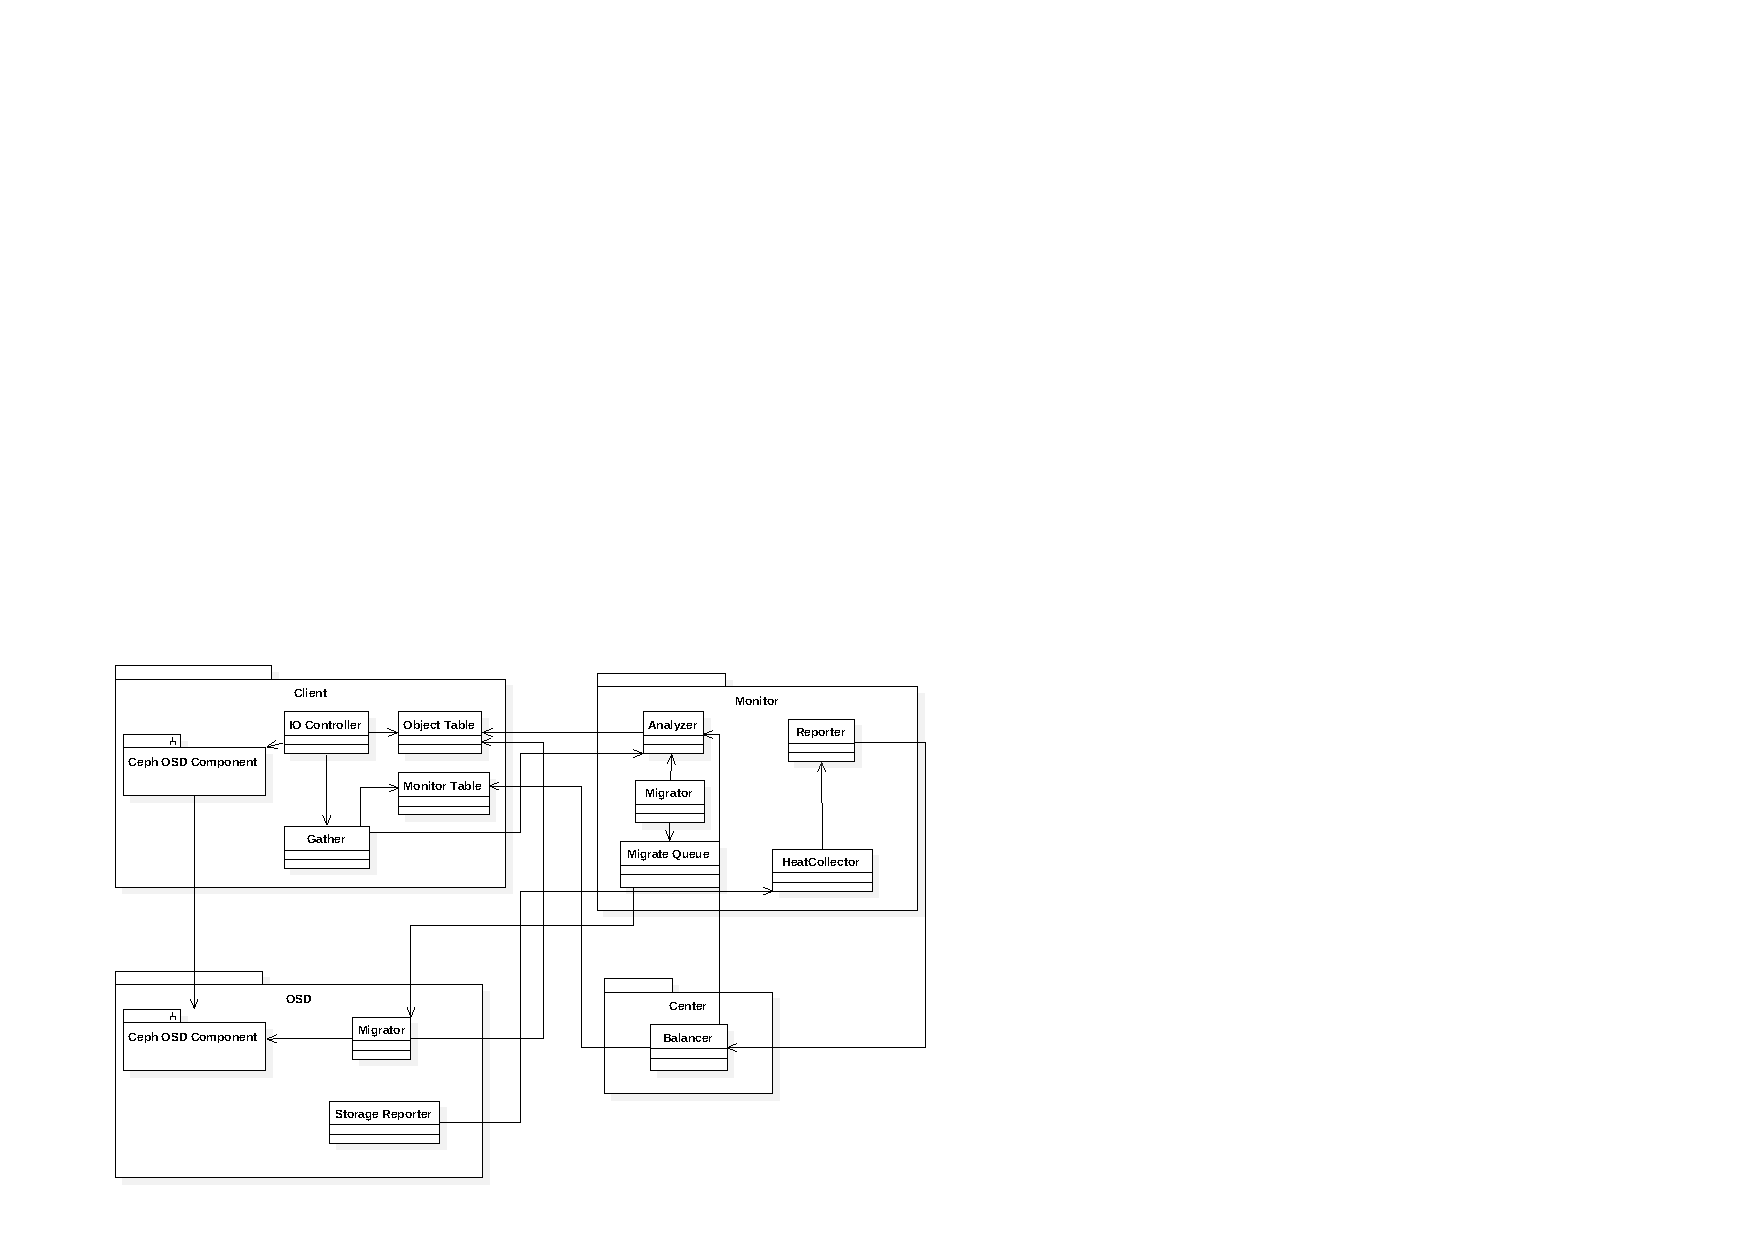
\includegraphics[width=15cm]{example/implmain.pdf}
    \bicaption[fig:implmain]{DOBBS模块结构}{DOBBS模块结构}{Fig}{Module Structure of DOBBS}
\end{figure}

Client主要包含四个类,这四个类也是与系统设计中的模块一一对应的。IO Controller用来截取VM的数据请求,并通过查询Object Table的方式来获取对象所在的OSD编号,再把对象ID和所在OSD编号共同
传递给Ceph OSD Component进行数据访问。IO Controller还有就是需要调用Gather的接口来记录VM访问对象的访问类型和ID,因此IO Controller没有暴露给外部的接口,它则主要对Ceph和QEMU源代码的修改。
Object Table的主要作用是保存一个对象ID到OSD ID映射的数据结构,并暴露出可以让IO Controller进行查询的接口,另外在局部热均衡对象迁移结束之后OSD上的Migrator也需要调用Object Table提供的更新映射的接口。
Gather则用于收集对象的访问信息,并调用Monitor上的接口将单位时间的数据流信息汇报给Monitor的Analyzer。而Monitor Table是用于存储Monitor ID与OSD ID的数据结构,因为全局热均衡会改变系统的逻辑结构,所以在全局热均衡结束之后会去更新Monitor Table提供的更新映射的接口。Gather则用于收集对象的访问信息,并调用Monitor上的接口将数据汇报给Monitor
,Gather在汇报给Monitor的之前需要先通过对象的OSD查询Monitor Table得到到该OSD在哪个子集群,然后在将相同子集群的对象数据流信息整合起来打包发送给对象的Monitor。

Monitor则包含五个类。Analyzer是用于接收Client的Gather所汇报的数据流信息,并且它内部会持续计算对象热度,在生成对象迁移策略之后调用Migrator发送迁移请求,Analyzer的另一个重要功能就是接受Center节点的命令开始热扩散的使能过程。
Migrator则主要负责对象的迁移请求发送等。Migrator Queue的主体是一个队列,用于存储迁移请求,另外Migrator Queue还会额外记录子集群当前迁移数量。Heat Collector是在全局热均衡中所用的类,它的主要作用是调用操作系统
指令获得Monitor的CPU和内存利用率,还有就是调用所在子集群OSD上的Storage Reporter接口获取存储设备的IOPS。Reorter则是会调取HeatCollector提供的接口获得实时子集群热度值,并定时将这个值
发送给Center的Balance。Center上的Balancer的主要功能就是接受Monitor发送的子集群热度值,然后运行算法\ref{algo:imbadect}生成热扩散请求,在热扩散结束之后再修改所有Client上的Monitor Table。


\subsection{Monitor的模块实现}
\begin{figure}[!htp]
    \centering
    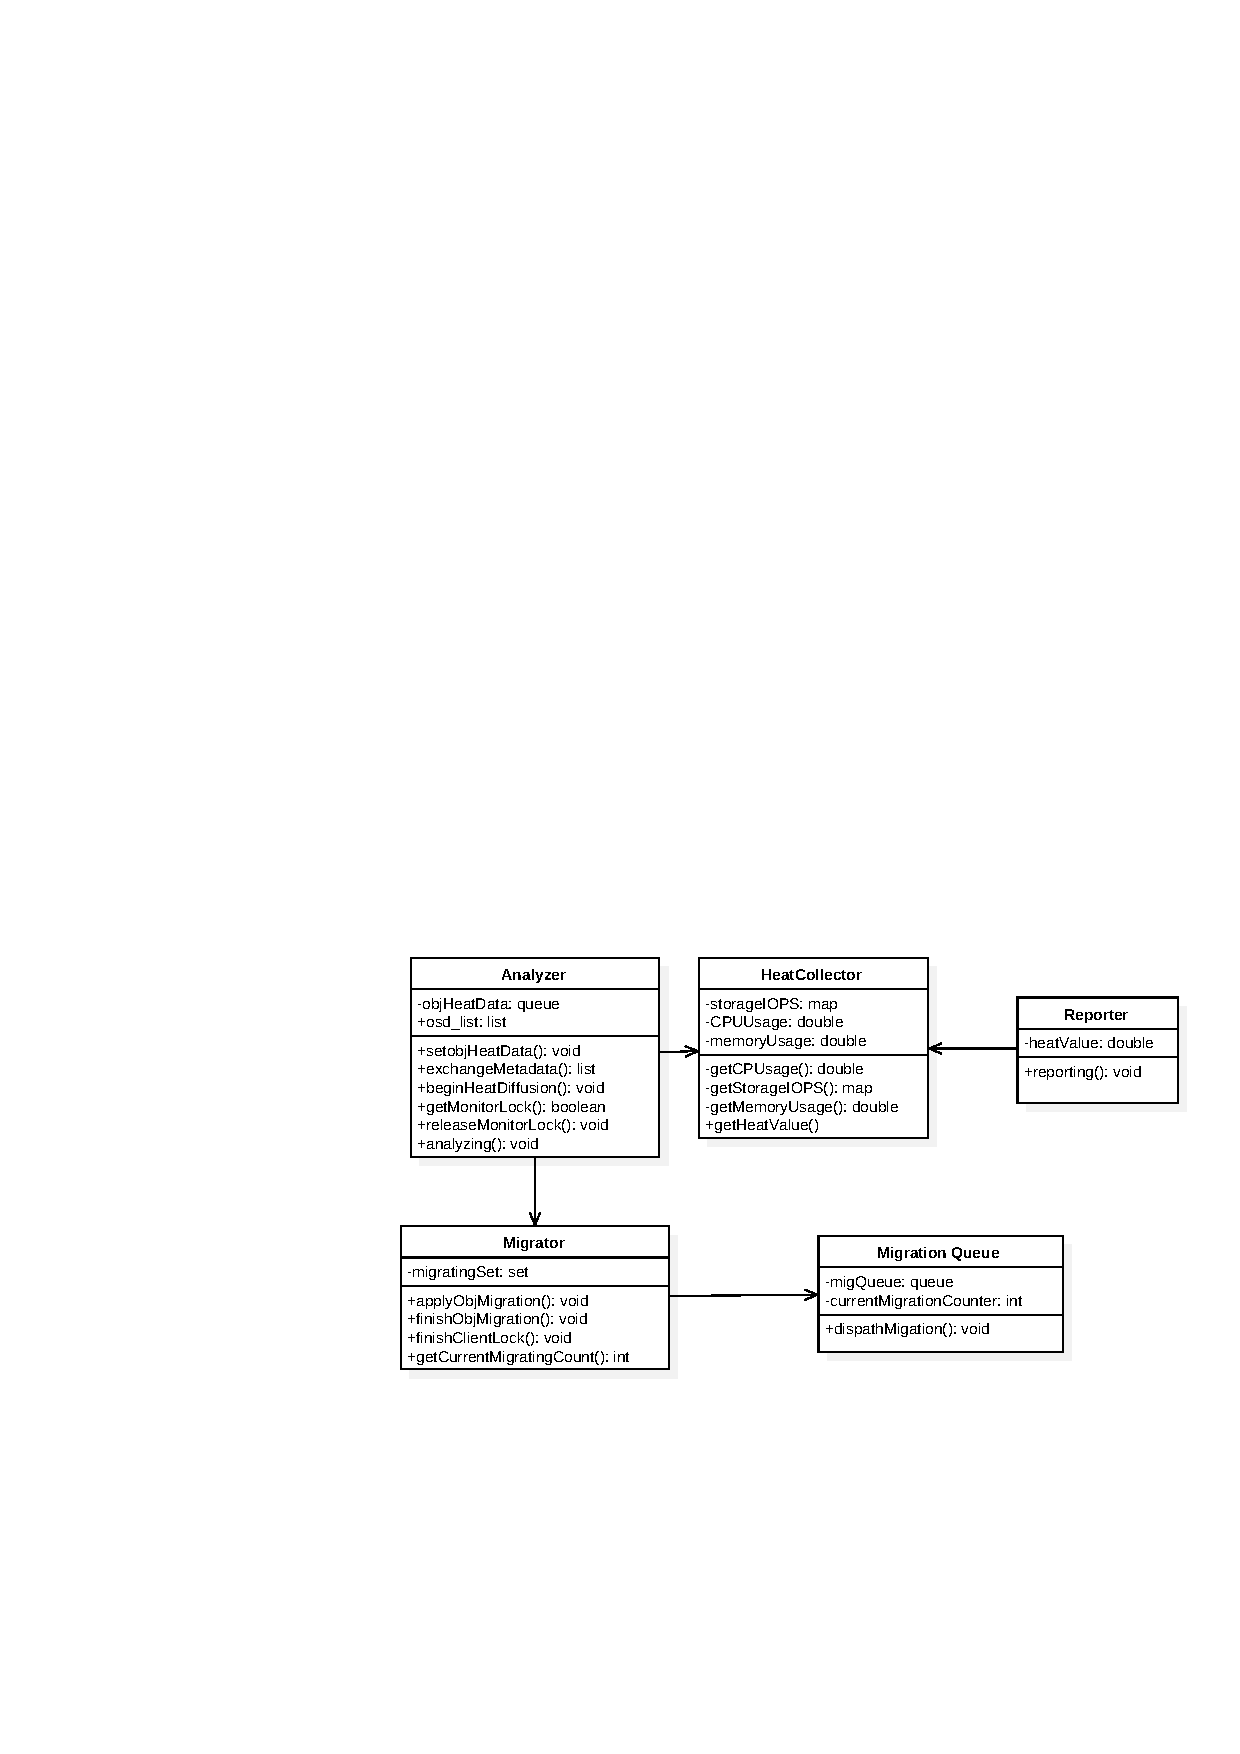
\includegraphics[width=14cm]{example/implmon.pdf}
    \bicaption[fig:implmon]{监视器模块类图}{监视器模块类图}{Fig}{Class Diagram of Monitor}
\end{figure}

图\ref{fig:implmon}所示是Monitor模块的设计类图。从图中可以看到Monitor一共有五个主要的类,其中的Analyzer、Migrator和Migrator Queue是继承于WHOBBS的实现\cite{lingxuan2015whobbs}。在本小结中,我们只做
简单的介绍,但是我们扩展了原有Analyzer类的功能,如全局热均衡的使能过程。

\subsubsection{Analyzer}
Analyzer的主要功能就是在局部热均衡的时候保存数据对象的热度信息,然后不断分析所有数据对象,计算对象的热度,并产生对象迁移请求。objHeatData是一个有序队列,我们实现了一个叫做ObjectQueue<typename T>的内置类,它内部是通过链表实现的
队列结构,只不过在链表插入的时候是根据元素的热度值进行的降序排序,保证了对头的元素的热度值总是最大的。objHeatData实际上的类型是ObjectQueue<ObjInfo>,ObjInfo是我们用来表示对象热度信息的结构体,这个结构体包含对象ID(oid)、所在
OSD编号(osd\_id)、所属Client IP(client\_ip)和热度(heat\_val)。因此objHeatData是用于存储对象热度信息的,它通过heat\_val降序排序。Analyzer还有个数据结构是osd\_list,它的类型是std::list<int>,它用来存储当前子集群所包含的OSD
编号。

analyzing()方法是一个线程入口函数,Analyzer在被实例化之后就会启动分析线程。分析线程工作就是不断遍历objHeatData,产生对象迁移请求。根据上一章对Monitor的设计,analyzing遍历时候的策略就是将会维护一个当前SSD剩余容量的计数,在SSD的容量
没有满的时候,它会把objHeatData的前若干个对象放置于SSD上。然后在该线程内部也会有两个集合,分别表示当前在SSD中的对象和在HDD中的对象。通过前面的策略,很快SSD就会被填满。
一旦SSD的容量已满,该线程则会遍历objHeatData的前N个对象,N的大小等于SSD容量/单个对象大小,找到这前N个对象中哪些是在SDD上哪些是在HDD上。如果出现HDD上的对象位于前N的位置,则将该对象从HDD迁移到SSD上。如果发现SSD集合中的对象不在前N的位置里,
则将该对象迁出SSD\cite{lingxuan2015whobbs}。该分析线程发送迁移指令是通过调用Migrator的applyObjMiration()的接口来实现的。setObjData()接口的实现相对简单,它只是用来在Monitor接收到Client汇报来的数据流对象,通过热度计算算法计算出每个对象的热度之后,如果objHeatData中含有这个对象
则更新它的热度值,否则实例化一个ObjInfo对象,将它插入到objHeaData中。值得注意的是,objHeatData的插入过程我们用到的是插入排序算法,从而保证每次插入都是有序的。

beginHeatDiffusion()、getMonitorLock()、releaseMonitorLock()和exchangeMetadata()这四个接口是Center所调用的。getMonitorLock()是用于对局部热均衡上锁,它会先去调用Migrator的getCurrentMigratingCount()接口获取现在子集群是否还有正在迁移的对象,如果接口返回值非0,则
不能上锁,接口返回false。如果getCurrentMigratingCount()的返回值是0,则会对analyzing()上锁并返回true,上锁我们是通过Linux的互斥锁pthread\_mutex\_t来实现的。beginHeatDiffion()接口是Center检测到子集群热度不均衡之后,并对Monitor
上锁之后执行的接口。这个接口就是全局热均衡使能过程的开始。而releaseMonitorLock()接口是Center在全局热均衡使能过程之后用于释放Monitor锁的,它调用pthread\_mutex\_unlock()这个Linux线程函数来解除加载analyzing线程上的互斥锁。这个互斥锁
是用在Analyzer的objHeatData这个数据结构上的,在上锁之后其他线程就不能对objHeatData进行读写操作,从而局部热均衡将被暂停。

beginHeatDiffusion()接口传入的参数是目标子集群Monitor的IP地址。在接口开始调用的时候,它会调用HeatCollector的getStorageIOPS()接口,这个接口会返回子集群的存储集群各个OSD的编号和IOPS的映射。在获得这个映射之后,它找到最大IOPS的OSD编号。
然后它会去objHeatData中去遍历,找到所有osd\_id为IOPS最大OSD的对象,将它们从队列中剔除并置于一个传输buffer中。这个buffer实际上类型为std::list<ObjInfo>的对象。封装完成后,它通过Thrift调用目标子集群Monitor的exchangeMetadata()接口以参数的方式将buffer中的元数据传输给目标子集群。目标子集群
会从接口exchangeMetadata()返回其最“冷”OSD所对应的元数据,返回值类型为std::list<ObjInfo>,然后将源子集群发送来的元数据调用setobjHeatData()接口插入objHeatData中。
beginHeatDiffusion()在接受到目标子集群的返回值之后,它把列表中的数据插入其自身的objHeatData,在接口执行的最后它会更新osd\_list中值,最后它调用Center的finishDiffusion()
方法,通知Center热扩散的使能过程已经完成。exchangeMatadata()接口则是在目标子集群的Monitor上被调用的接口,它的参数是源子集群最“热”OSD对应的元数据。该接口被调用之后,它会通过查询HeatCollector,找到IOPS最低的OSD编号,并将它所对应的元数据从onjHeatData中剔除,并通过返回值的方式传送给源子集群。

\subsubsection{Migrator和Migrator Queue}
Migrator和Migrator Queue的实现与WHOBBS中的实现相似,我们这里不再详细叙述这两个模块的实现。Migrator主要向Analyzer提供applyObjMigration()接口,Analyzer调用该接口后,该接口的传入参数是一个表示对象迁移的数据结构,它包括被迁移对象的原OSD编号、目的OSD编号和对象ID,
,然后它会调用Client上的对象上锁接口,在上锁成功后将迁移请求(表示迁移的数据结构)放置于Migrate Queue。
finishObjMigrating()接口是在OSD结束对象传输之后调用的,调用之后会把这个对象从migratingSet中剔除,然后调用Client上的释放锁的接口\cite{lingxuan2015whobbs}。与WHOBBS不同的是,为了支持Monitor锁,我们增加了getCurrentMigratingCount()接口,这接口在调用之后会直接返回当前migratingSet的大小。
migratingSet是在发送请求之后将oid放入其中,直到迁移完成后才会把它从migratingSet删除掉,因此migratingSet表示的是当前正在迁移对象的ID。Migrator Queue的实现与WHOBBS无异,本文则不再叙述。

\subsubsection{HeatCollector}
HeatCollector的功能是获取子集群的所有事实资源信息的。它主要有三个成员变量,分别是storageIOPS(存储集群IOPS)、CPUUsage(Monitor的CPU利用率)和memoryUsage(Monitor的内存利用率)。其中storageIOPS的数据类型是std::map<int, long>,这个map数据结构的键为osd\_id,值为对应OSD的IOPS值。
CPUUsage和memoryUsage的类型都是double,即占用百分比。

getHeatValue()是HeatCollector对外提供的接口,该接口被调用之后,它会依次调用getStorageIOPS()、getCPUUsage()和getMemoryUsage()接口获得当前实时的子集群资源信息,并更新它的三个成员变量。对于getStorageIOPS(),它会从在Analyzer的osd\_list获取子集群所包含OSD的编号,
然后再调用本子集群的OSD上的getIOPS()接口,最后将最新的存储集群IOPS值以map的方式返回。getCPUUsage()接口则是调用Linux的系统调用查看/proc/stat文件来获取当前CPU利用率。getMemoryUsage()则调用sysinfo()系统调用来获得当前的内存利用率的。在getHeatValue()成功调用这些接口
之后,它会根据公式\ref{eq:stheat}计算当前实时的热度值并返回给调用者。

\subsubsection{Reporter}
Reporter的功能则是汇总子集群的资源利用信息,并定时发送给Center。Reporter包含一个成员变量,就是当前子集群的实时热度是heatValue,它的类型是double。reporting()函数是一个线程入口函数,该线程的主要功能就是不断的调用HeatCollector的getHeatValue()接口,在每次获取之后都会调用Center的reportFromMonitor()接口把热度值传输给Center。

\subsection{Center模块实现}

\begin{figure}[!htp]
    \centering
    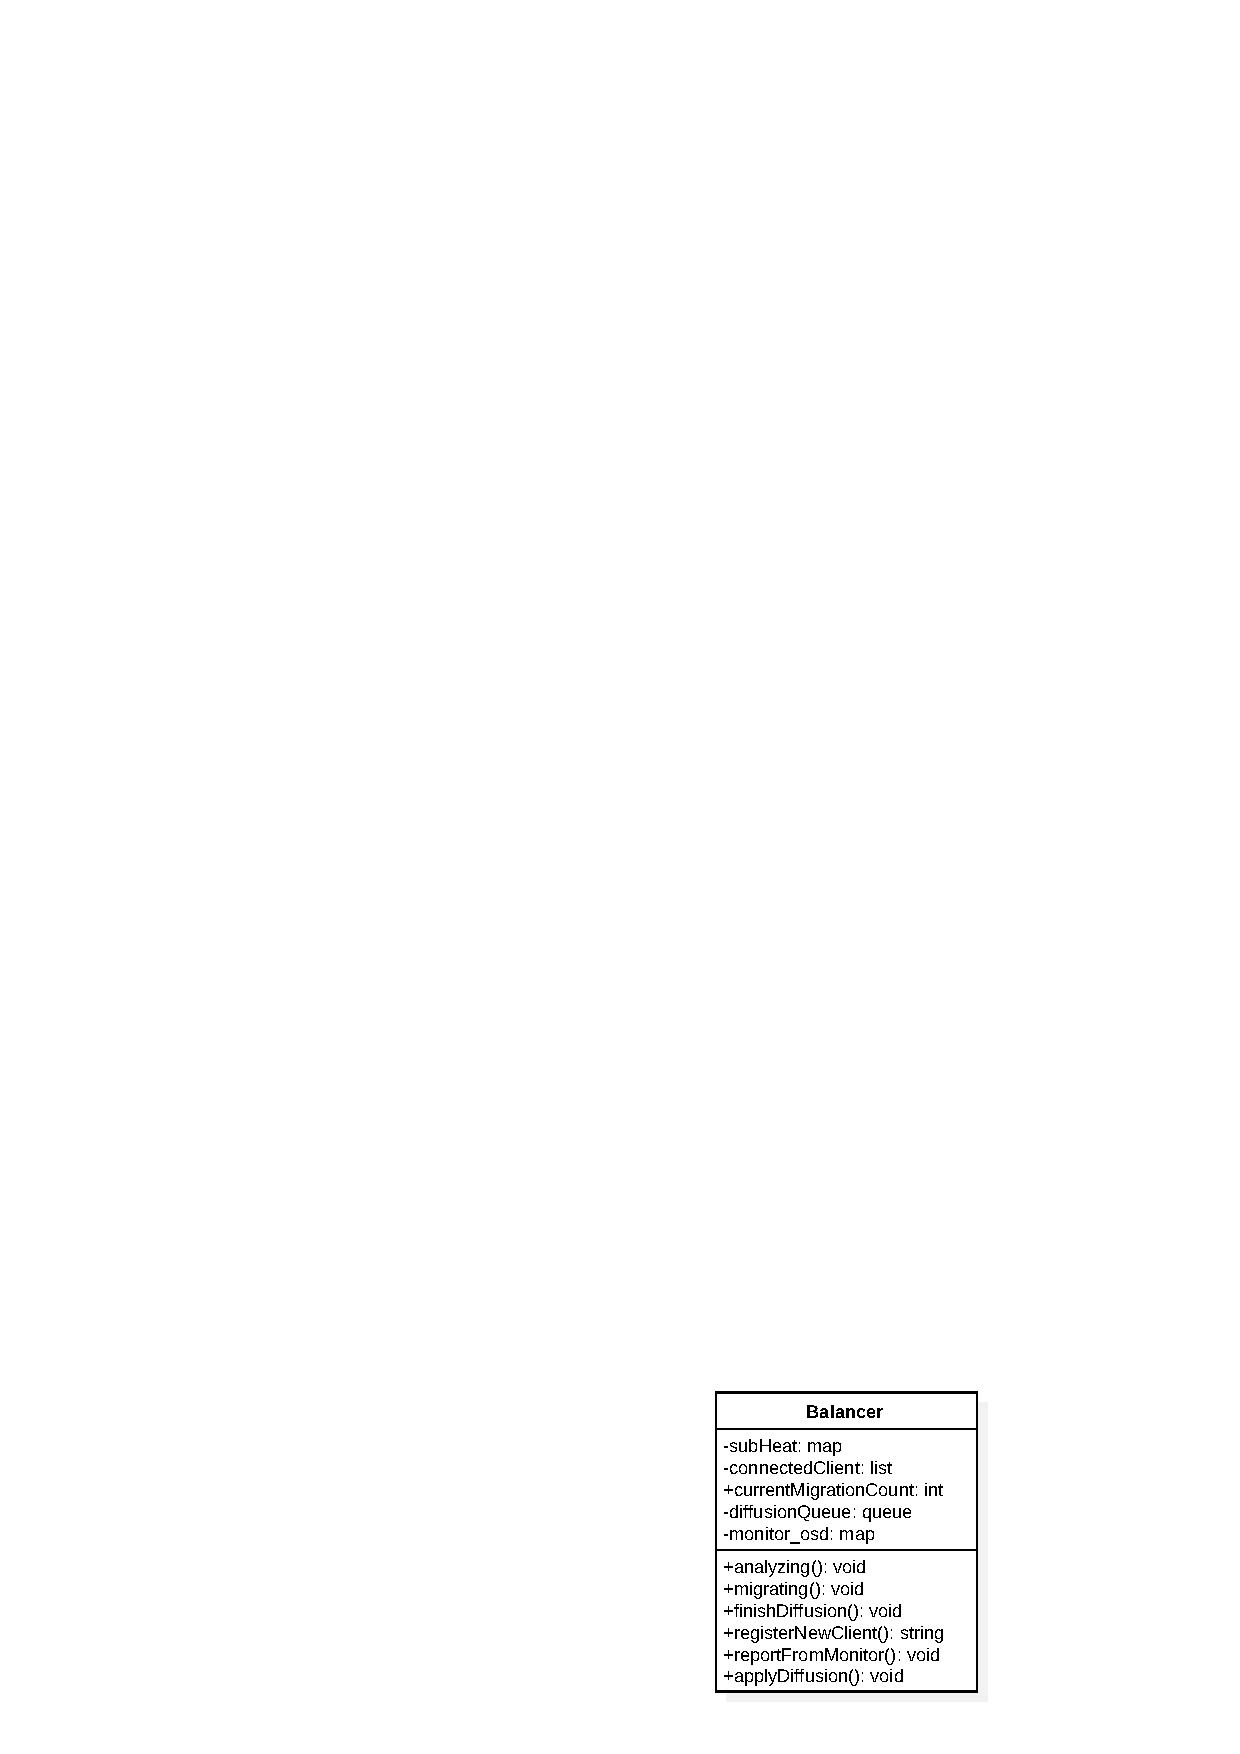
\includegraphics[width=5cm]{example/implcenter.pdf}
    \bicaption[fig:implcenter]{中心模块类图}{中心模块类图}{Fig}{Class Diagram of Center}
\end{figure}

如图\ref{fig:implcenter}所示为DOBBS的Center模块的类图,从图中可以看到Center只有一个叫做Balancer的类。Balancer类就实现了Center的所有功能,包括对各个子集群热度信息的收集、产生热迁移请求和新Client接入时的分配。

\subsubsection{Balancer}
Balancer主要有subHeat、connectedClient、currentDiffusionCount、diffusionQueue和monitor\_osd等五个成员变量。subHeat的数据类型的std::<std::string, double>,它表示各个子集群的热度值,其中的键为子集群id,值为热度值。connectedClient,它的类型是
std::list<std::string>表示当前接入系统的Client的IP地址。currentDiffusionCount表示当前正在全局热均衡的请求数量,它的类型是int。diffusionQueue表示准备进行热扩散的队列,它的类型是std::queue<DiffusionDetail>,DiffusionDetail是一个用来表示热扩散请求的结构体,
它包含to\_sub和from\_sub,即源子集群和目标子集群的编号。

Balancer的analyzing()函数是一个线程入口函数,这个线程主要就是用来运行子集群热度不均衡检测算法\ref{algo:imbadect},当算法找到源子集群和目的子集群之后会把原子群和目标子集群标号通过参数的方式传递给接口applyDiffusion()。而analyzing线程会过一定时间间隔
执行一次热度不均衡检测算法。reportFromMonitor()接口则是用于持续接受,各个Monitor所汇报的热度值信息。

applyDiffusion()算法在接收到源子集群编号和目标子集群编号之后,会生成一个DiffusionDetail类型的结构体,该结构体包含to\_sub(目标子集群)、from\_sub(源子集群)这两个信息,并将其放置于diffusionQueue中。migrating()函数则是迁移线程的入口函数,它的工作就是不断轮训diffusionQueue的内容,只要队列不为空它
会先检查currentDiffusionCount的值是否达到系统最大热扩散数量,如果已经达到则不对队列做任何处理。如果currentDiffusionCount小于系统最大热扩散数量,那么它会通过子集群编号调用两个子集群的getMonitorLock()接口,只有当两个都返回true时才将
这个热扩散请求从diffusionQueue删除。在这之后,它会调用源子集群的beginHeatDiffsion()接口,并将目标子集群标号传递给它。

finishDiffusion()接口是在源子集群和目标子集群结束全局热均衡的使能过程之后调用的,最终是由源子集群调用。在调用之后,Center会首先更新monitor\_osd的值,因为全局热均衡已经修改了子集群的逻辑结构。然后,Center再去更新通过connectedClient列表
去更新所有连接的Client的MonitorTable。最后则是调用目标子集群和源子集群的releaseMonitorLock()接口对两个Monitor解锁。

在上一章已经讲过,当Client初次接入系统时,Center会分配一个相对较“冷”的子集群给这个Client。在Client初次接入时,它会调用registerNewClient()接口,再把自己的IP地址通过传参的方式发送给Center。这个接口会遍历subHet,找到一个热度值最低的
子集群,然后将这个子集群Monitor的id返回给Client,最后Center把这个Client的IP置于connectedClient中。

\subsection{Client模块实现}
\begin{figure}[!htp]
    \centering
    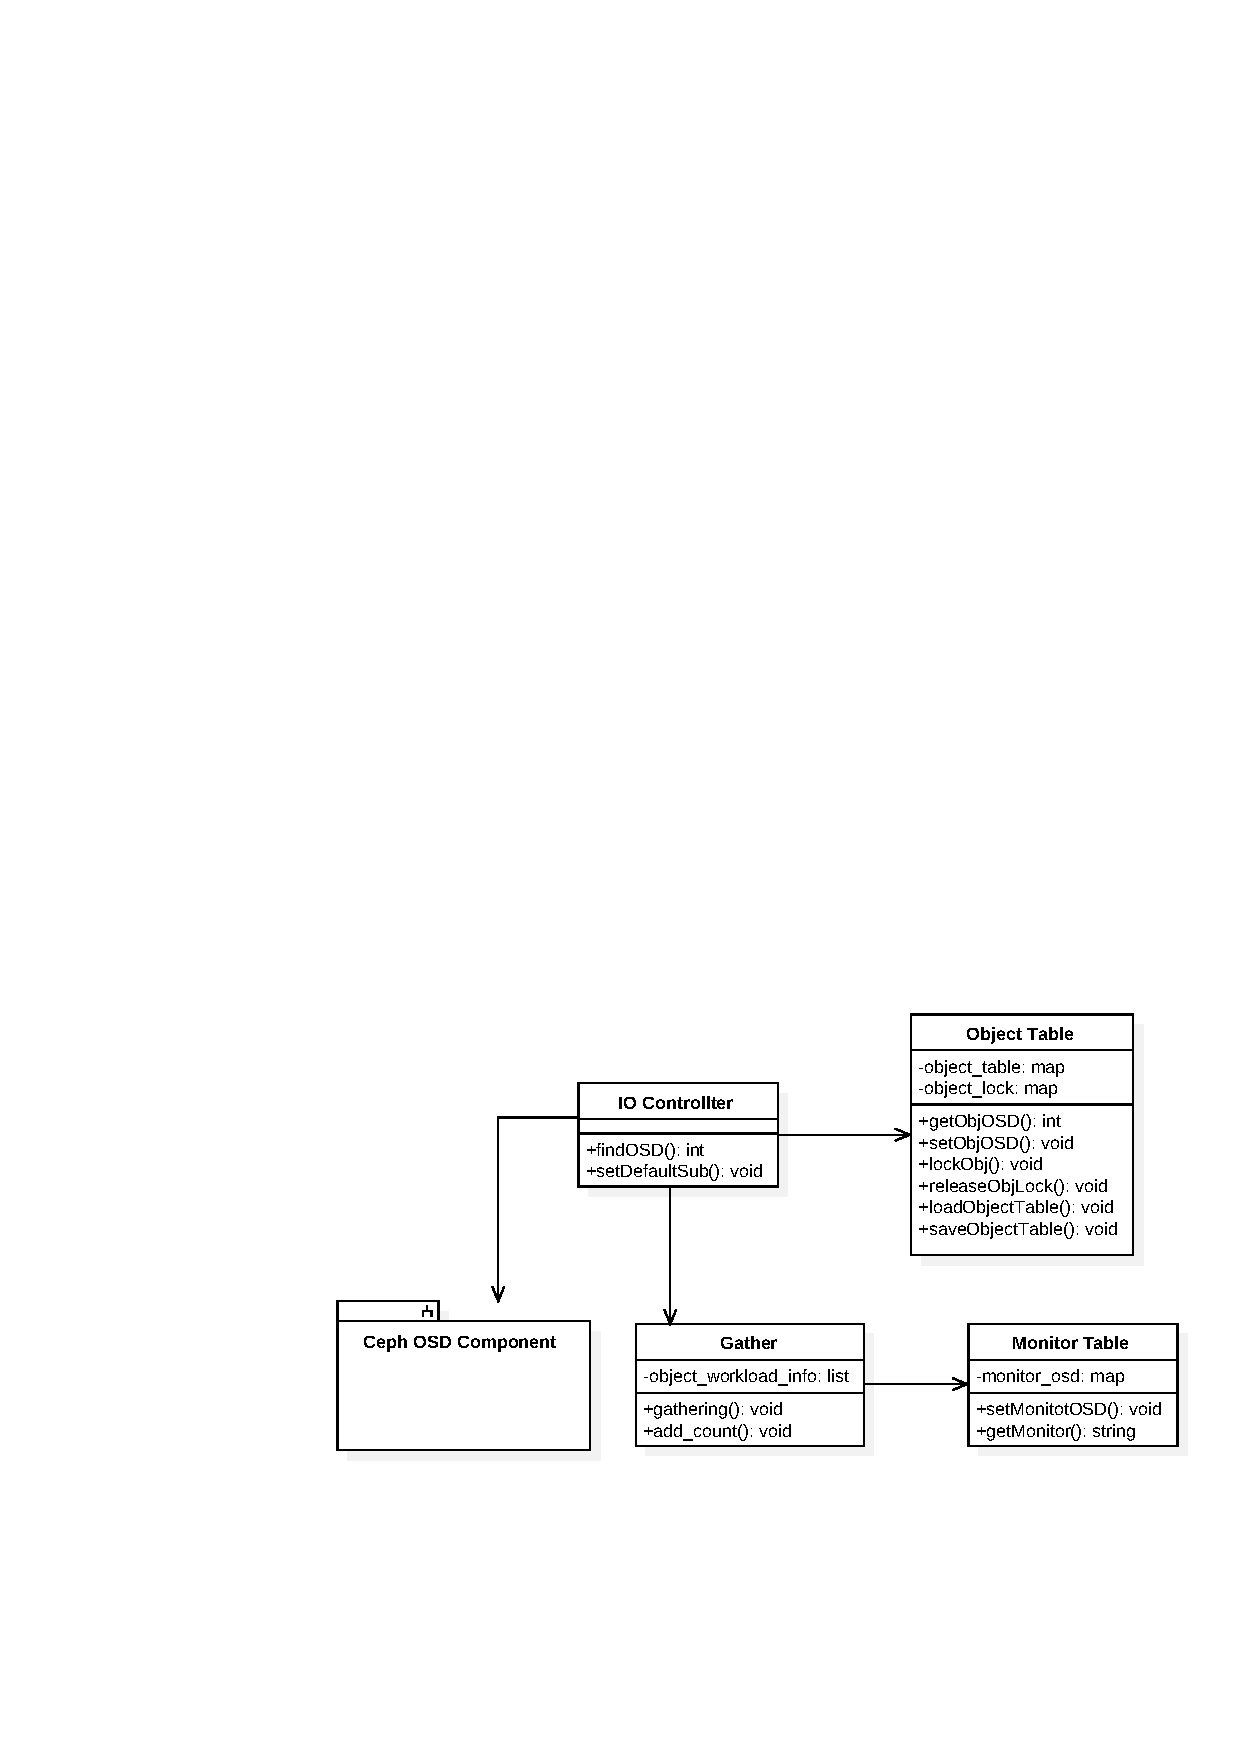
\includegraphics[width=12cm]{example/implclient.pdf}
    \bicaption[fig:implclient]{客户端模块类图}{客户端模块类图}{Fig}{Class Diagram of Client}
\end{figure}

如图\ref{fig:implclient}为Client模块的类图。Client模块是运行虚拟机和虚拟机管理器的模块,该模块的IO Controller、Object Table和Gather这三个类的实现与WHOBBS基本一致,所以本文不再过多赘述。但是,我们在原有实现的基础上加入了Monitor Table类,用于负责全局热均衡后系统的OSD和Monitor之间
的变化。

因为Client的设计,我们要截取VM对对象访问的请求,这就需要我们对Ceph的原生代码做出修改。我们主要修改了Ceph librbd模块的代码,在Ceph调用底层对象传输之前,我们让它先调用IO Controller的findOSD()接口。IO Controller的findOSD()接口是以对象ID
作为参数,然后在Object Table中调用getObjOSD()接口进行查询对象当前所对应的OSD编号,然后返回给Ceph之后,再进行后续的对象访问。值得注意的是,因为DOBBS的多Monitor设计,以及静态全局热均衡,所以我们需要在Client初次接入系统的时候可以获得它所在的默认
子集群。因此,与WHOBBS不同,我们在IO Controller加入了一个接口setDefaultSub()这个是用于Center设置当前Client默认子集群的接口。当然,为了在Client第一次接入DOBBS才会去向Center获得默认子集群编号,我们也对Ceph的源代码进行了修改。

Object Table的实现与WHOBBS没有区别,本文仅介绍各个接口的作用,具体细节不再介绍。首先,该类包含两个成员变量,分别是object\_table和object\_lock。它们都是std::map的数据结构,object\_table是用来保存对象ID和OSD编号的映射关系,而object\_lock并
不保存信息,只是保存哪些对象上了锁。而getObjOSD()和setObjOSD()则是对object\_table进行操作,分别是通过对象ID获取对应的OSD编号,还有就是修改object\_table的内容。lockObj()和releaseObj()这两个接口都是在局部热均衡过程中保证一致性对对象上锁和解锁
所用到的接口。loadObjTable()和saveObjTable()则是用于在DOBBS系统启动和关闭后将object\_table存盘和读取的接口。

我们在WHOBBS原有Gather类的基础上进行了扩展。gather()是线程入口函数,它的功能就是定时向Monitor发送对象的数据流信息。我们定义对象的数据流信息包括,对象ID(oid)、OSD ID(sid)、访问类型(access\_type)、访问次数(access\_count)。与WHOBBS不同,在WHOBBS中只有一个
Monitor存在,所以所有Client都只需要向同一个Monitor发送自己的数据流信息。对于DOBBS,我们的Monitor会有多个,而且由于全局热均衡,OSD也会随之发生变化。在DOBBS的设计中,OSD是与子集群绑定的,所以我们需要保证Client可以实时知道每个OSD都在哪个子集群中。
Monitor Table就是用来保存子集群和OSD的信息。gather线程在每次向Monitor发送之前,都会通过Monitor Table查询到当前对象所在的OSD位于哪个子集群,然后将相同子集群的对象数据流信息组合成一个列表共同发送给对应的Monitor。

Monitor Table类的主要功能,首先是保存当前最新的OSD和子集群的信息,其次就是接受来自Center的更新,还有就是Gather会来查询。它有一个叫做monitor\_osd的成员变量,它的类型是std::map<std::string, std::string>,它存储了OSD ID到子集群Mointor的IP地址之间的映射关系。
setMonitorOSD()接口是由Center远程调用的,在全局热均衡的使能过程之后Center会通知所有连接到系统的Client更新各自的Monitor Table。getMonitor()接口则是开放给Gather用于查询对象所在子集群的,它传入的参数是OSD ID,返回值为Monitor的IP地址。

\subsection{OSD模块实现}
对于OSD模块的实现,我们完全沿用了WHOBBS的实现方案没有做更多的扩展,所以本小节只做简要的概括。可以从图\ref{fig:implmain}中看到,OSD上的Migrator负责接收来自于Monitor的迁移请求,在接收到之后,它只需要调用Ceph的OSD组件即可完成对象的迁移。而Storage Reporter则是调用了
操作系统指令获得当前磁盘(SSD/HDD)的IOPS值。Monitor上的Heat Collector类会远程调用Storage Reporter的接口获得当前的IOPS值。

\section{系统主要工作流程}
本小结主要介绍DOBBS的主要工作流程。局部热均衡中的工作流程,如对象的迁移、对象数据流信息的获取以及虚拟机的IO请求这些工作流程与WHOBBS中的实现并没有太大的区别,所以本小节对局部热均衡的工作流程只是做一个高度的概括,而不做过多的描述。
全局热均衡是一个复杂的过程,我们将它抽出三个比较主要的工作流程来进行介绍,分别是客户端接入工作流程、监控器获得并汇报子集群热度信息工作流程和全局热均衡使能过程工作流程。客户端接入过程,是静态的全局热均衡的保证并且还是让
客户端可以顺利与系统交互的重要保证。监控器获得并汇报子集群热度信息的过程也就是Center获得各个子集群热度的过程,这对Center进行子集群热度不均衡检测尤为重要。全局热均衡使能过程是全局热均衡最重要的一环,本小结从Center发出
迁移指令开始来叙述全局热均衡的使能过程。

\subsection{局部热均衡工作流程}

局部热均衡的工作流流程主要可以分为以下几个部分:虚拟机IO请求工作流、虚拟机汇报对象数据流信息工作流以及对象迁移工作流。虚拟机IO请求工作流一般是由虚拟机发起的,然后IO Controller先去查询Object Table,找到该对象对应的
OSD ID,然后将OSD ID返回给IO Controller,最后IO Controller将对象ID和OSD ID以参数的方式调用Ceph OSD Component接口,来进行后续的访问。在这个过程中,IO Controller起到的是截取请求的作用。值得注意的是,因为我们要
获得对象的访问信息,所有在IO Controller的findDefaultOSD()被调用的时候,它还会调用Gather的add\_count()接口,把当前虚拟机所访问的对象ID和访问类型传递给Gather。


虚拟机汇报对象数据流信息工作流则相对简单,Gather的gathering线程会定时将储存的对象数据流信息发送给Monitor的Analyzer,而每次发送之后它都会清空之前的记录。对象迁移工作流则是局部热均衡的重点。Analyzer在得出迁移策略之后,它会
调用Migrator,Migrator生成迁移请求,然后Migrate Queue把迁移请求缓存下来,如果子集群当前的迁移数量小于最大迁移数量则开始迁移。首先,调用Client上的lockObj()接口,之后向该对象对应的OSD发送请求,OSD调用Ceph OSD Component进行
对象迁移,迁移结束后OSD调用Migrator的finishObjMigration()接口,最后再对Client上的对象解锁。

\subsection{客户端接入工作流程}
\begin{figure}[!htp]
    \centering
    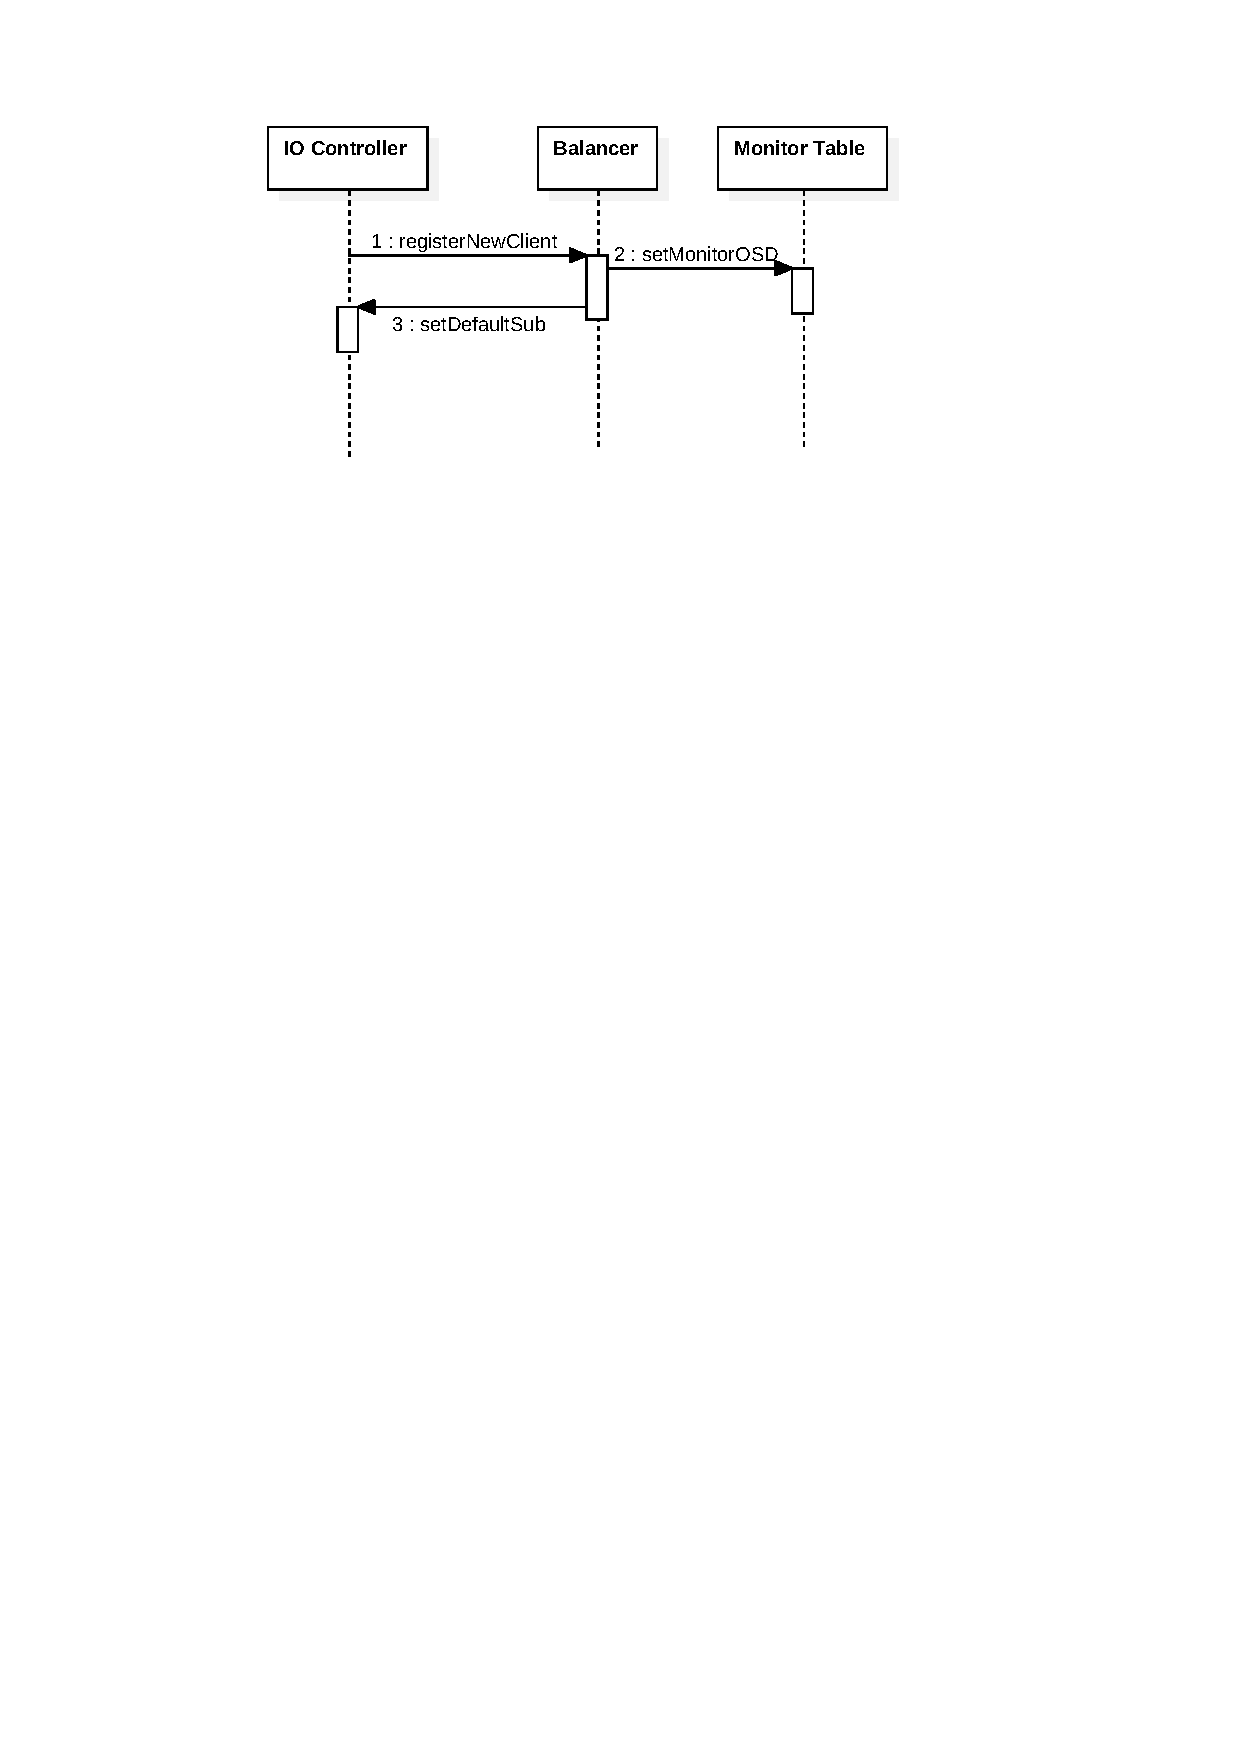
\includegraphics[width=10cm]{example/seqinit.pdf}
    \bicaption[fig:seqinit]{客户端接入的工作流程}{客户端接入的工作流程}{Fig}{The Work Flow of Client First Access}
\end{figure}

客户端初次接入DOBBS的工作流程如图\ref{fig:seqinit}所示。从图中可以看到,IO Controller会首先调用Center的Balancer的registerNewClient()接口,然后该接口通过查询subHeat,将当前热度值最低的子集群发送给IO Controller。同时,
它会把请求接入的Client的IP地址写入connetedClient中,然后把当前系统最新的monitor\_osd通过调用setMonitorSub()发送给这个初次接入的Client。

\subsection{监控器获得并汇报子集群热度信息工作流程}

图\ref{fig:seqhet}所示,是子集群的Monitor向Center发送当前子集群热度值的工作流程,这个工作流程还包括Monitor的HeatCollector定期从子集群的OSD中获取IOPS信息,并根据
公式\ref{eq:stheat}计算子集群热度,最后再把计算好的热度值通过Thrift提供的远程调用接口发送给Center。

对于该工作流,值得注意的是Reporter发起的getUsage请求是由Reporter的reporting线程发送的,reporting线程则是以固定的时间间隔发起getUsage请求。HeatCollector在收到请求
之后,会先去在Analyzer上去查询本子集群有哪些OSD。在这之后,它会通过查询到的OSD列表调用每个OSD上的getStorageIOPS()接口,接口返回后,HeatCollector将其记录并依次调用getCPUUsage()
和getMemoryUsage()接口,最后通过公式计算出热度值并调用Center的reportFromMonitor()接口将它传输给Center。

\begin{figure}[!htp]
    \centering
    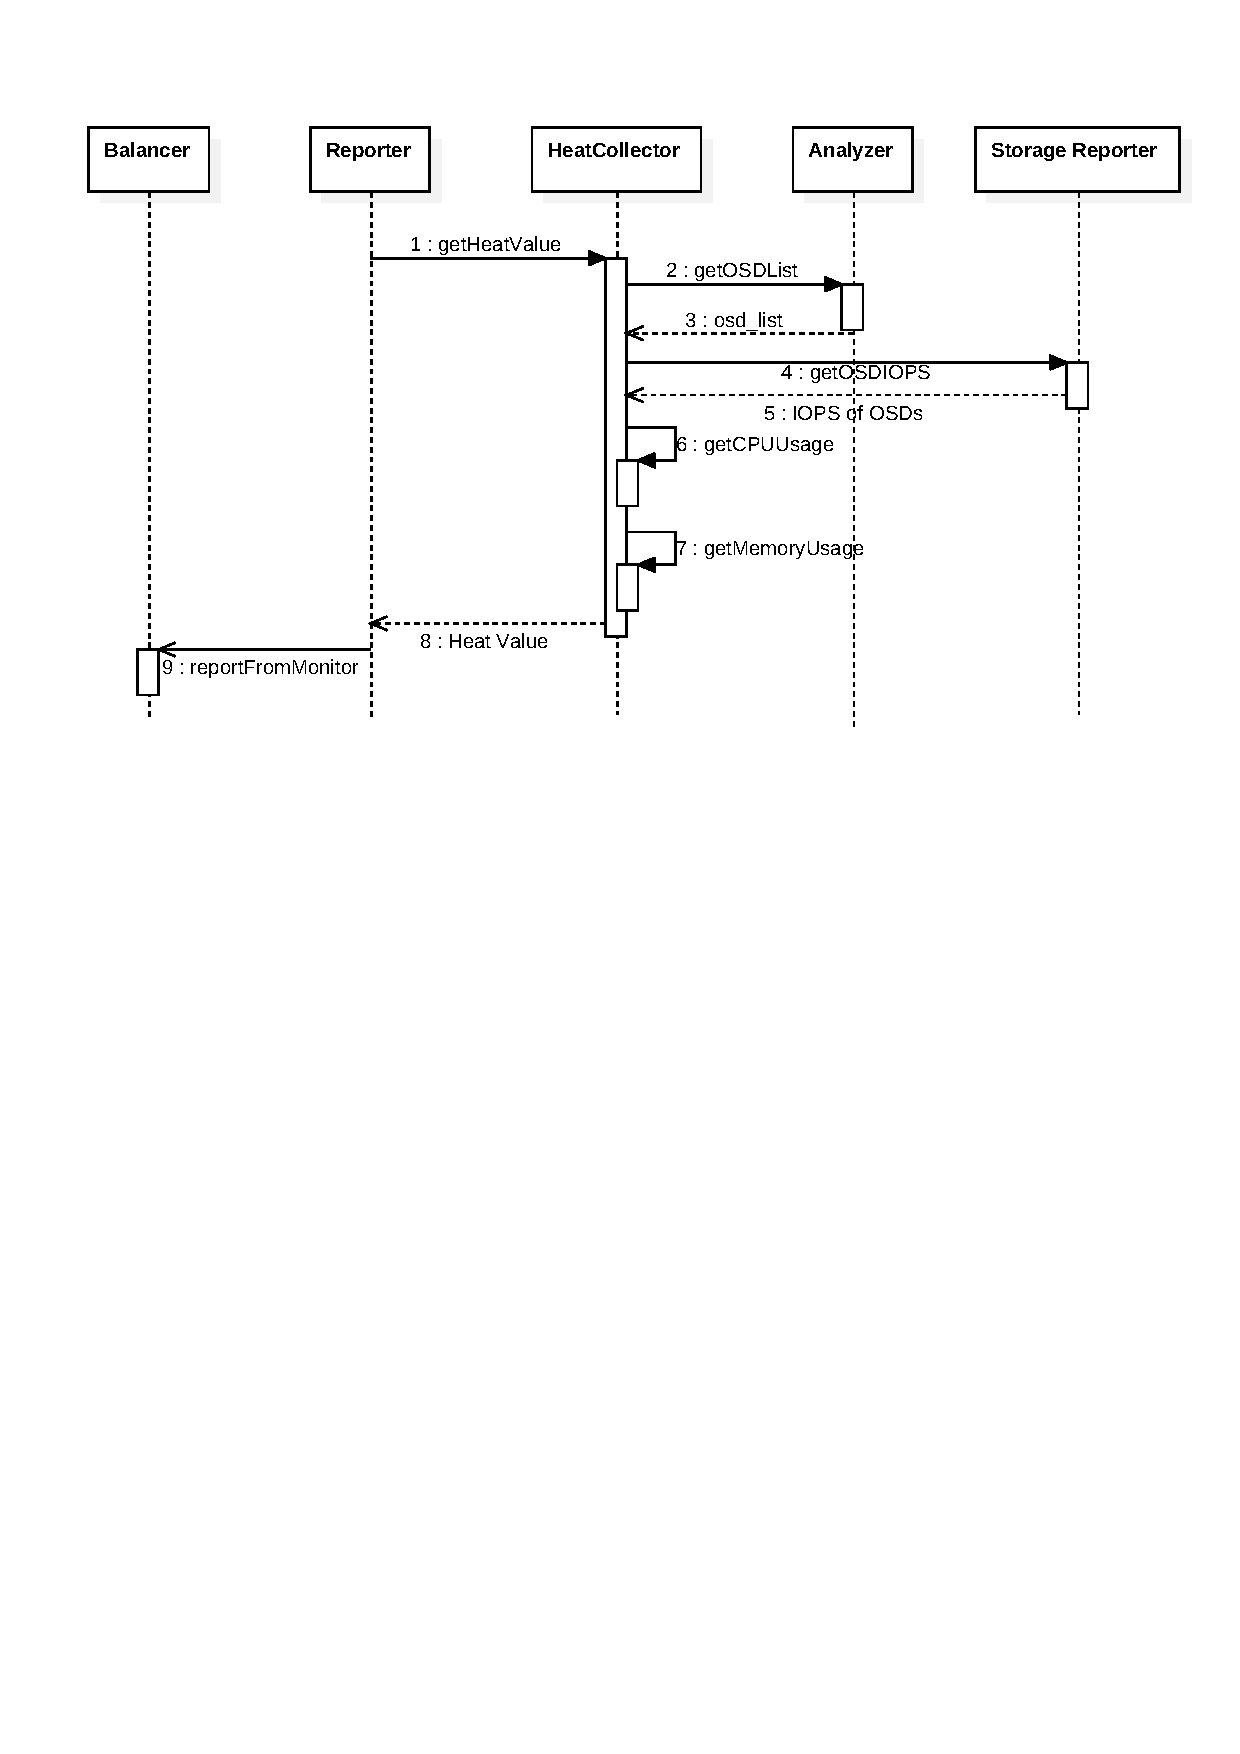
\includegraphics[width=12cm]{example/seqhet.pdf}
    \bicaption[fig:seqhet]{监控器获得并汇报子集群热度信息工作流程}{监控器获得并汇报子集群热度信息工作流程}{Fig}{The Work Flow of Monitor Reports Heat}
\end{figure}

\subsection{全局热均衡使能过程工作流程}


全局热均衡是本论文的一个核心概念,而全局热均衡的使能过程更是关键。图\ref{fig:seqghb}所示为全局热均衡的使能过程的工作流程。在Balancer的不均衡检测算法检测出不均衡之后,就
启动了使能过程。首先就是为了解决迁移过程中的一致性问题,我们用try-lock机制来对Monitor上锁。但是图\ref{fig:seqghb}中,我们假设的是成功上锁之后的工作流程。如果不能成功地从
目标子集群和源子集群获得锁,则不会进行后续的使能过程。
\begin{figure}[!htp]
    \centering
    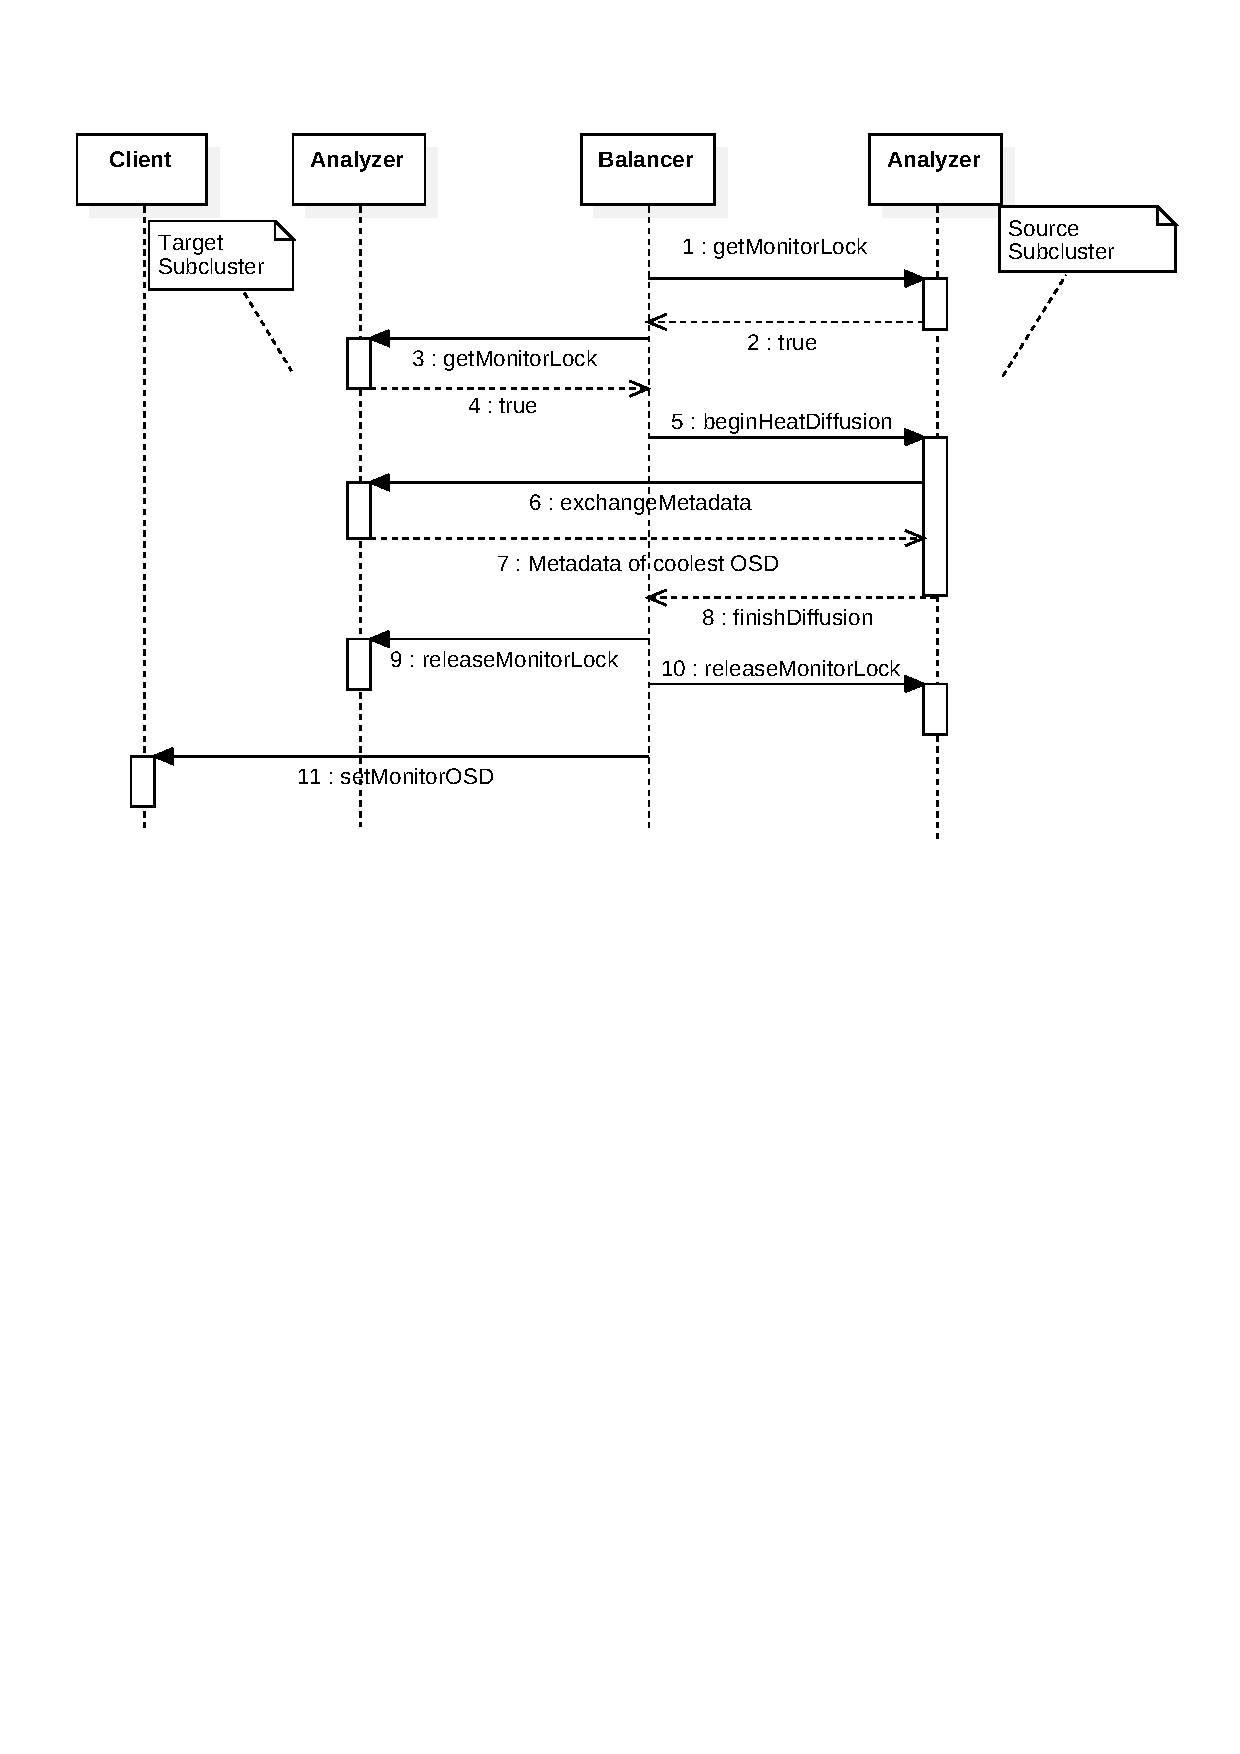
\includegraphics[width=12cm]{example/seqghb.pdf}
    \bicaption[fig:seqghb]{全局热均衡使能过程工作流程}{全局热均衡使能过程工作流程}{Fig}{The Work Flow of Enable Process of Global Heat Balancing}
\end{figure}
在成功获得两个Monitor的锁之后,Balancer会调用源子集群Monitor的Analyzer的beginHeatDiffusion()接口。之后,源子集群会查询最大IOPS的OSD然后将其对应的元数据(对象热度信息)打包
发送给目标子集群,通过目标子集群的exchangeMetadata()接口。目标子集群再去查询当前子集群IOPS最低的OSD,将该OSD对应的元数据返回给源子集群。在所有过程完成之后,源子集群再调用Balancer的
finishDiffusion()接口,完成元数据交换。随后,Balancer对两个子集群的Monitor解锁。最后则是更新所有Client上的Monitor Table。

\section{本章小结}
本章基于上一章设计的基础上对DOBBS的系统各个模块的设计进行了介绍。首先,我们介绍了DOBBS构建过程所用到的工具和开源项目,主要有Ceph、QEMU和Apache Thrift。我们选用的主要开发语言为C++。本章
第二小节,我们首先介绍了DOBBS的各个模块的类图框架,然后对各个模块分别展开了叙述。因为DOBBS是在WHOBBS的基础上进行的扩展和修改,所以我们对WHOBBS部分的实现并没有做出详细的叙述。本章第三小节则是
对系统的主要工作流程的抽象与总结。我们对全局热均衡的主要三个流程进行了详细的介绍。下一章,则是根据本章所实现的系统做出实验验证。

